\section{議論}

\subsection{『わかるらんど』の思想}

近年、学会などでタイムライン表示のテキストチャットが
利用される機会が増えている\cite{WISSのチャットの報告論文}。
学会チャットシステムを利用すると、
発表中に参加者が意見交換したり疑問を表明したりできるといった利点があるが、
以下のような問題も存在する。

\begin{itemize}
\item 多数の人間が同時に投稿すると投稿内容がすぐに見えなくなってしまう
\item 投稿の多いアクティブな人ばかりが目立ってしまい、消極的な参加者は議論に参加しにくい
\end{itemize}

一般に、会議などで特定の人だけが沢山発言するのはよくあることであるが、
誰もが気軽に意見を表明できる環境を構築できれば有意義であろう。

日本ソフトウェア科学会主催の
WISS (Workshopn on Interactive Systems and Software)コンファレンス\footnote{
  \textsf{http://wiss.org/}
}では、
学会が提供するチャットシステムに参加者がログインして
議論するのが恒例になっており、
2009年以降のWISSコンファレンスでは
「On Air Forum」\cite{OnAirForum}という
学会チャットシステムが利用されている。
%
しかし、
WISS2009の実証実験\cite{nishida2011}によれば、
全参加者の半分弱しかログインして1回以上発言していなかった。
またWISS2015では、252アカウントが1回以上発言し総発言数は2,948回であったが、
発言数上位20\%の50アカウントによる発言が総発言数の78.1\%にあたる2,305回を占めていた(図\ref{wisschat})。
また、発言数が10回未満のアカウントは190アカウントで、これは全アカウントの75.3\%にあたる。

\begin{figure}[h]
\centering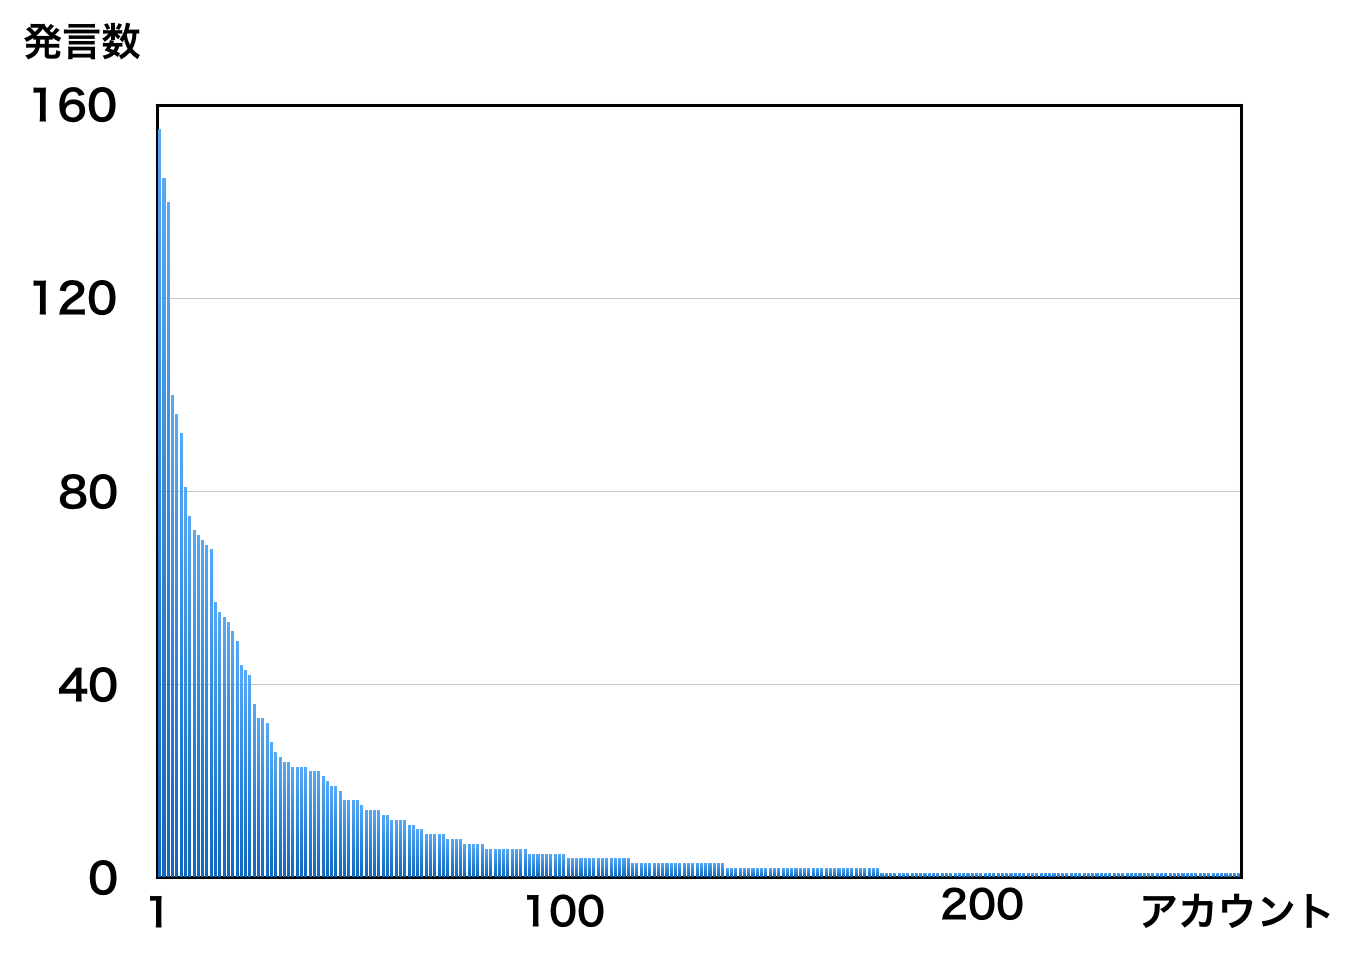
\includegraphics[width=8cm]{images/wisschat.png}
\caption{WISS2016のチャットにおけるアカウント毎の発言数}
\label{wisschat}
\end{figure}

『わかるらんど』はユーザの表示領域が均等に決まっているため、
タイムライン表示のように投稿数が多い人ばかりが目立つということがない。
また、長いテキストを入力すると表示される文字が小さくなるので、
150人程度で利用すると長い文字は小さすぎて読めない。
必然的にユーザは図\ref{wakaruland150}のように短文を入力することを強いられる。
『わかるらんど』では長文の高度な発言は期待しておらず、
「なるほど」「わからん」「笑」などといった相槌のようなものを
視覚化してひと目で把握できるようになることを期待している。
学生、先生、企業に所属する人等様々なバックグラウンドの人が入り混じった状況で
「下手な発言ができない」「気の利いたことを言わなければならない」という
投稿を躊躇させる要素を限りなく減らし、
本当は議論に参加したいけど声が出ない/手を上げる勇気がない人でも
「なるほど」「わかる」などを『わかるらんど』に投稿することで「参加」することができる。
テキストで記述すると長くなってしまう内容も
画像スタンプを投稿することで分かってもらうことができると考える。

\comment{
また、長いテキストを投稿するには適していないので『わかるらんど』を使って議論することは難しいが、
多くの会議やコンファレンスでは発表後に議論の時間が設けられているため議論はその時に行えばよい。
}

\begin{figure}[h]
\centering
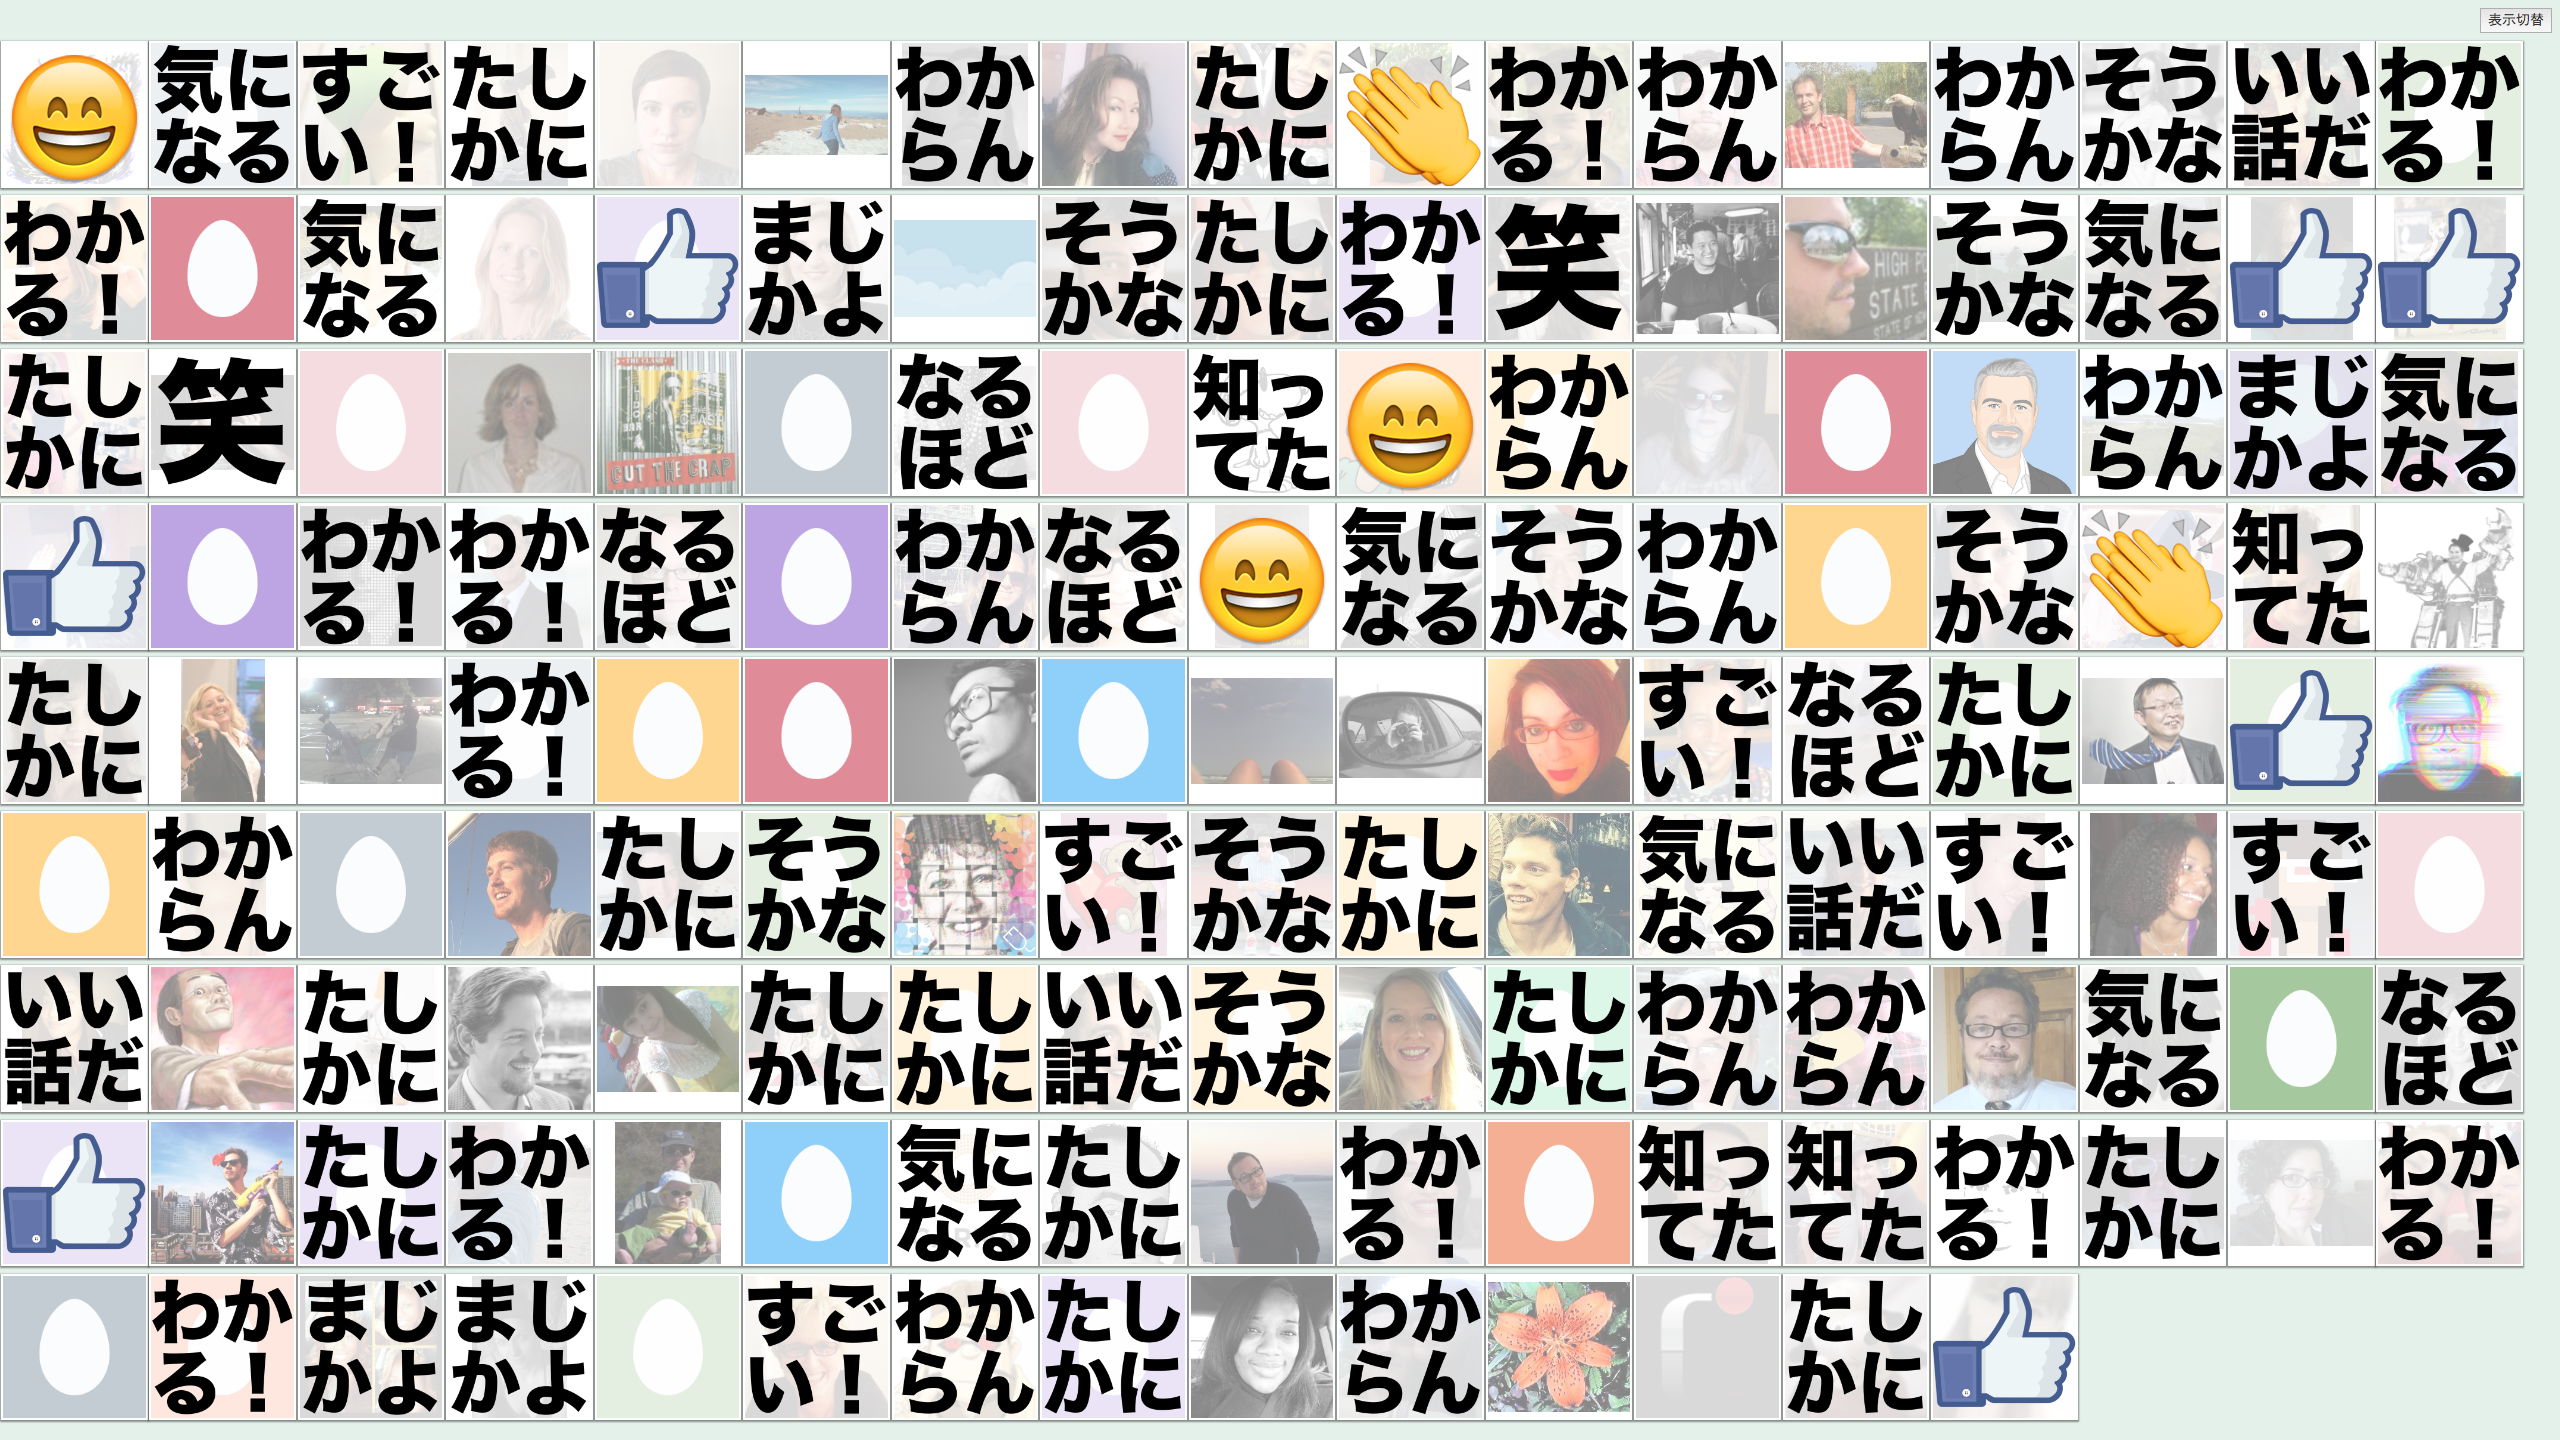
\includegraphics[width=8cm]{images/wakaruland150.png}
\caption{150人で『わかるらんど』を使用したイメージ}
\label{wakaruland150}
\end{figure}

\subsection{研究室においての利用経験}
我々の研究室ではWebLindaを使用して、
\begin{itemize}
\item 部屋の明るさを知る
\item 部屋の温度を知る
\item 風速と風向を知る
\item 入口のドアの鍵を開ける
\item 部屋の照明を点ける/消す
\end{itemize}
をSlack\footnote{https://slack.com}のチャットボットを通じて行えるIoT環境を構築しているが、
『わかるらんど』と組み合わせることでさらに便利に使うことができた。

図\ref{light}は部屋の明るさを表示するデータセルだが、
明るさのデータの値が小さい時は\texttt{background}画像を変更することで、
照明が点いているのか消えているのかがわかるようになった。

\begin{figure}[h]
\centering
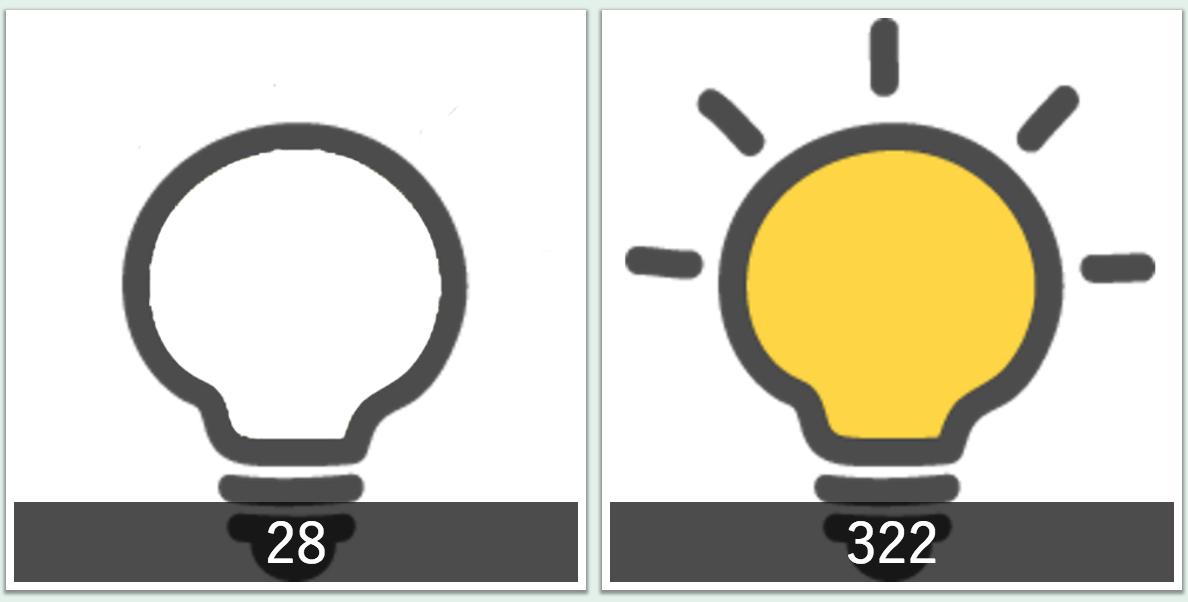
\includegraphics[width=7cm]{images/light.png}
\caption{照明が消えている時(左)と注いている時(右)}
\label{light}
\end{figure}

図\ref{door}は、研究室のドアが最後に開いた時間を表示するデータセルである。
普段は扉の画像をtexttt{background}にしているが、
実際に扉が開いた時に10秒間だけtexttt{background}を図\ref{door}右のように
扉を開ける人の画像にすることで、誰かが入室したことが視覚的にわかるようになった。

\begin{figure}[h]
\centering
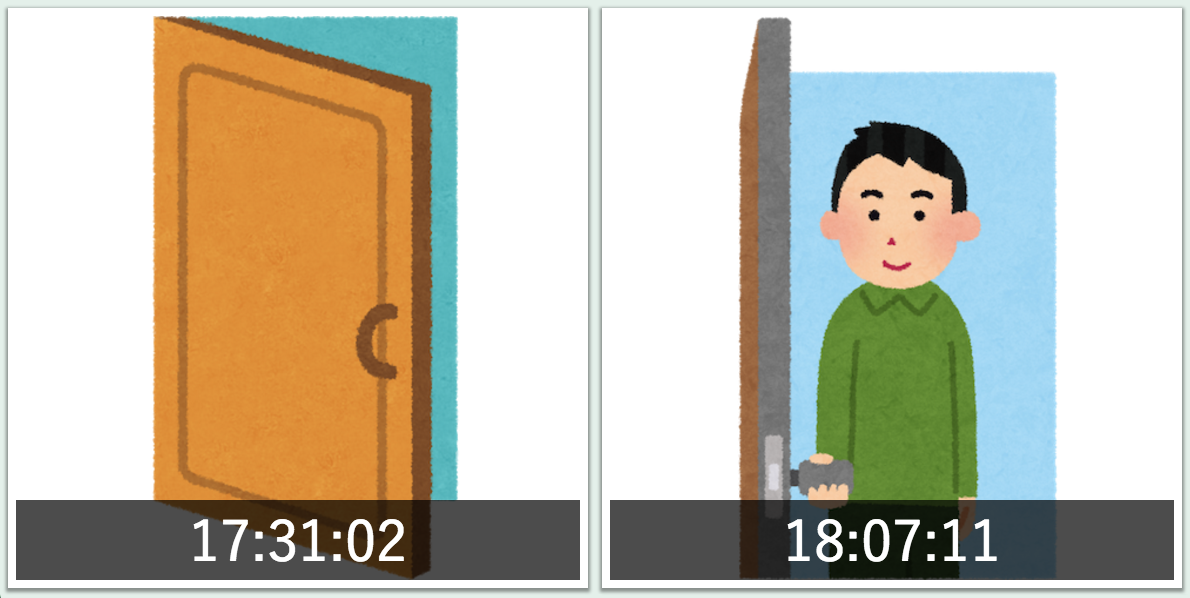
\includegraphics[width=7cm]{images/door.png}
\caption{ドアの普段の表示(左)と誰かが入室した時(右)}
\label{door}
\end{figure}

ミーティングの時間には積極的に『わかるらんど』を利用し、
普段発言の少ない人でも何らかの反応を表明したり、
発表者が聴衆の反応をひと目で把握することができるようになった。
誰かが面白いことを言ったときに「笑」というリアクションが並ぶなど、
『わかるらんど』を通じて一体感が生まれることもあった(図\ref{wara})。

\begin{figure}[h]
\centering
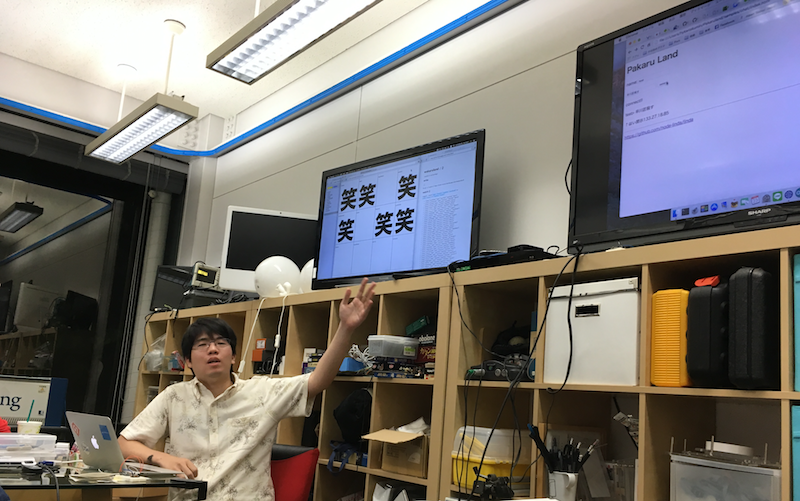
\includegraphics[width=7cm]{images/wara.png}
\caption{『わかるらんど』を使用したミーティング}
\label{wara}
\end{figure}